\documentclass{beamer}

\usepackage{amsmath,amssymb,amsfonts}
\usepackage{graphicx}
\usepackage[round]{natbib}
\usepackage{booktabs}
\usepackage{hyperref}
\usepackage{setspace}
\usepackage{lmodern} % for better font rendering
\usepackage{caption} % for table captions
\usepackage{adjustbox} % to resize tables if needed
\usepackage{multirow}
\usepackage{tcolorbox}

\usetheme{Madrid}
\usecolortheme{default}

% For references in footnotesize
\setbeamertemplate{bibliography item}[text]

\title[Generative AI and Job Displacement]{Generative AI and Job Displacement:\\
Initial Evidence from EU Online Job Markets}
\author[Georgi Demirev]{\textbf{Georgi Demirev}\\Sofia University}
\date{\today}

\begin{document}
% -------------------------------------------------------------------
\begin{frame}
    \begin{figure}
        
\includegraphics[width=0.45\linewidth]{img/StopanskiFakultet-Logo2.jpg}
    \end{figure}
    \titlepage
\end{frame}

% -------------------------------------------------------------------
\begin{frame}{Outline}
  \tableofcontents
\end{frame}

% -------------------------------------------------------------------
\section{Introduction and Motivation}
\begin{frame}{Humans need not apply}
    \begin{columns}
        \begin{column}{0.48\textwidth}
          \textbf{Worries about AI-induced job displacement are widespread}
          \begin{itemize}
            \item 60\% of white-collar workers fear AI automation \citet{oliverwyman2024generative}
            \item 1/3 of managers are redesigning workflows to reduce their dependency on people \citet{mercer2024global}
            \item 10\% of service companies reported laying off workers due to AI (vs 5\% reporting hiring new workers) \citet{nyfedsurvey2024}
          \end{itemize}
        \end{column}
        \begin{column}{0.48\textwidth}
            \begin{figure}
                \centering
                % Include your .png or .pdf instead of .eps if needed
                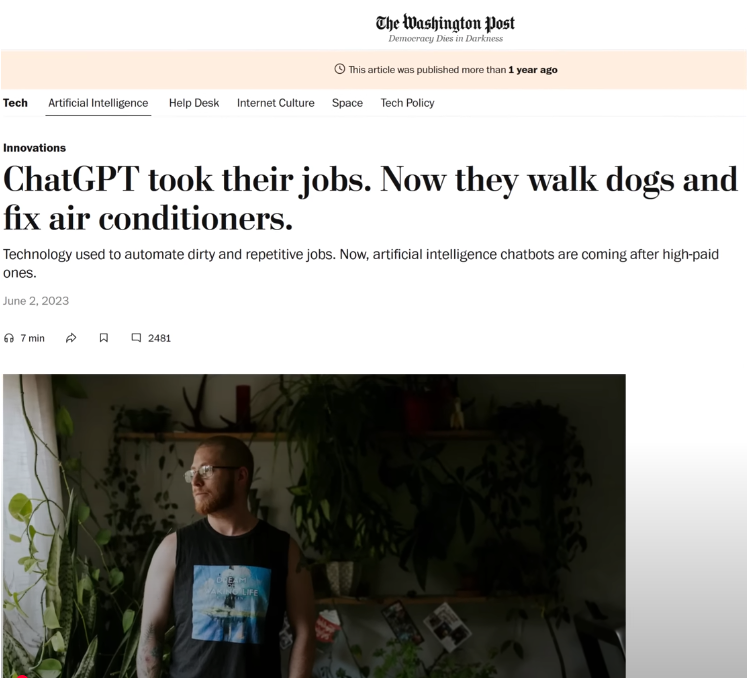
\includegraphics[width=0.95\textwidth]{img/slidesp/walk_dogs.png}
                \label{fig:headline}
            \end{figure}
        \end{column}
    \end{columns}
\end{frame}

\begin{frame}{Research Question}
    \textbf{Are jobs with higher exposure to AI experiencing worse labor market outcomes relative to jobs with lower exposure to AI?}

    \vspace{0.5cm}
    \begin{itemize}
        \item Data for occupational "AI exposure" from four independent studies
        \item Change in online job adverts as main outcome variable
        \item Additional outcomes on sectoral productivity and within-occupation skill demand
        \item Difference-in-difference with continuous treatment design
    \end{itemize}
\end{frame}

\begin{frame}{Key Findings}
\begin{itemize}
    \item Occupations with higher AI exposure experienced a \textbf{13--18\% larger decrease} in job postings relative to less exposed ones.
    \item Within occupations, skills most similar to AI capabilities saw a \textbf{10\% reduction} in mention frequency.
    \item No significant impact on capital or labor productivity was detected at the industry level so far.
\end{itemize}
\end{frame}

% -------------------------------------------------------------------
\section{Theoretical Framework}
\begin{frame}{Tasks and Automation}
    \begin{figure}
        \centering
        % Include your .png or .pdf instead of .eps if needed
        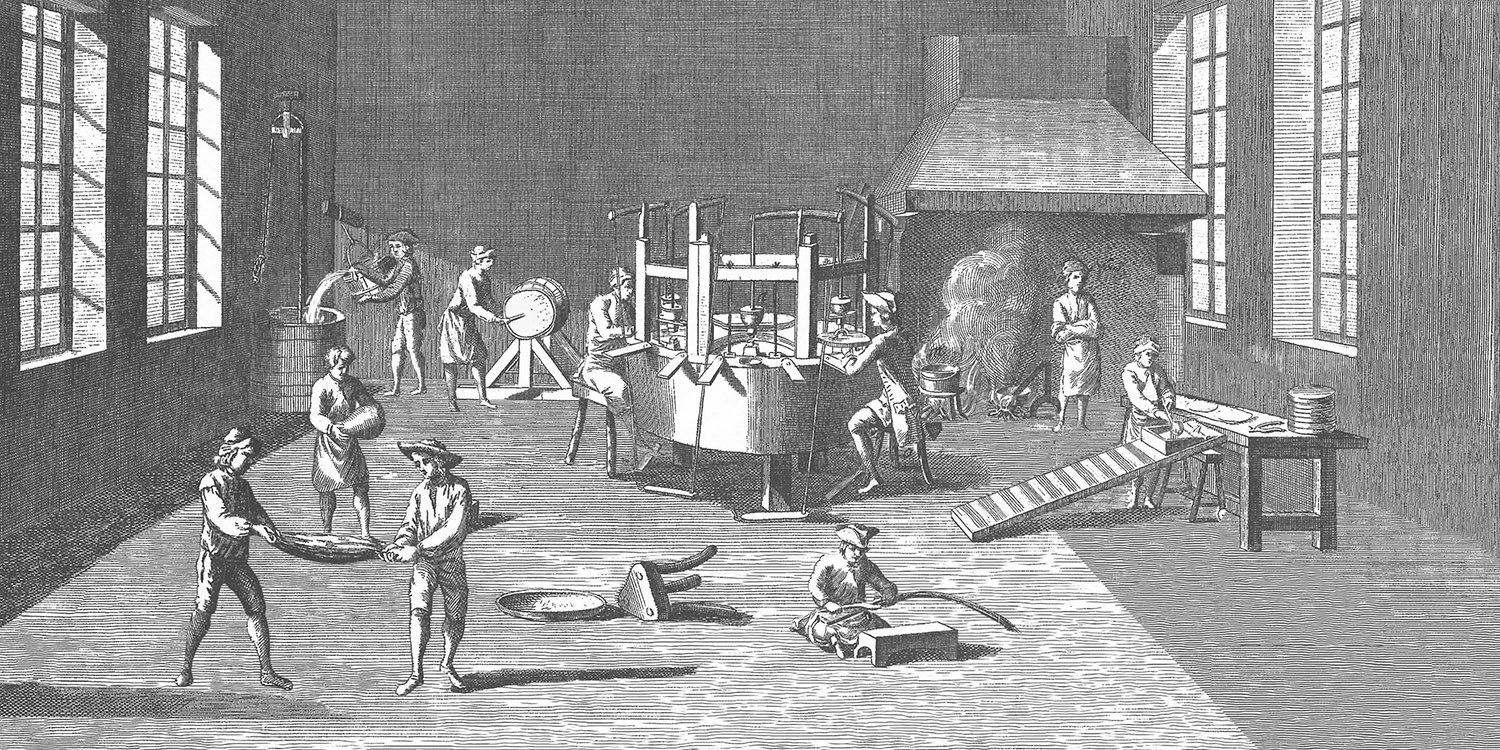
\includegraphics[width=0.95\textwidth]{img/pin_factory.jpg}
        \label{fig:pins}
    \end{figure}
    \begin{itemize}
        \item Task-based models of economic growth (\cite{zeira1998workers}, \cite{acemoglu_automation_2019}) view production as a sequence of interdependent tasks.
        \item $\ln{y_s}=\ln{A_s}+\int_{T_s}\alpha(x)\ln{y_s(x)}dx$
    \end{itemize}
\end{frame}

\begin{frame}{Theoretical Predictions}
    \begin{itemize}
        \item \textbf{Labor Augmentation} - when technology makes labor more productive, e.g. new tools or methods.
        \item \textbf{Capital Deepening} - improvement in parts of the process that are already performed by machines.
        \item \textbf{New Tasks} - novel labor-intensive steps in the production process enabled by newer production methods
        \item \textbf{Automation} - direct replacement of labor with machines.
        \begin{itemize}
            \item Welfare effects depend on the magnitude of the increase in productivity.
        \end{itemize}
    \end{itemize}
\end{frame}

% -------------------------------------------------------------------
\section{Data and Methods}
\begin{frame}{O*NET Classification}
    \begin{columns}
        \begin{column}{0.48\textwidth}
          \begin{figure}
                \centering
                % Include your .png or .pdf instead of .eps if needed
                
\includegraphics[width=0.95\textwidth]{img/slidesp/ee_anime.png}
                \label{fig:ee1}
            \end{figure}
        \end{column}
        \begin{column}{0.48\textwidth}
            \begin{figure}
                \centering
                % Include your .png or .pdf instead of .eps if needed
                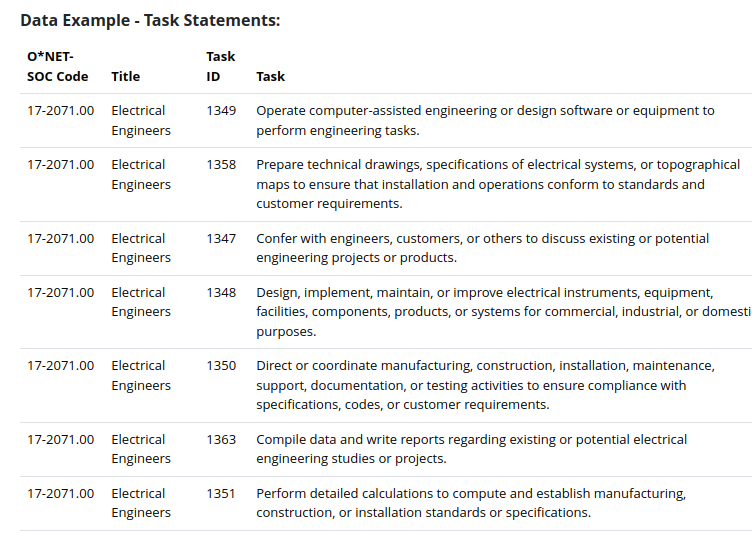
\includegraphics[width=0.95\textwidth]{img/slidesp/EE_ONET.png}
                \label{fig:onet_eng}
            \end{figure}
        \end{column}
    \end{columns}
\end{frame}

\begin{frame}{ESCO Classification}
    \begin{columns}
        \begin{column}{0.48\textwidth}
          \begin{figure}
                \centering
                % Include your .png or .pdf instead of .eps if needed
                
\includegraphics[width=0.95\textwidth]{img/slidesp/ee_anime.png}
                \label{fig:ee2}
            \end{figure}
        \end{column}
        \begin{column}{0.48\textwidth}
            \begin{figure}
                \centering
                % Include your .png or .pdf instead of .eps if needed
                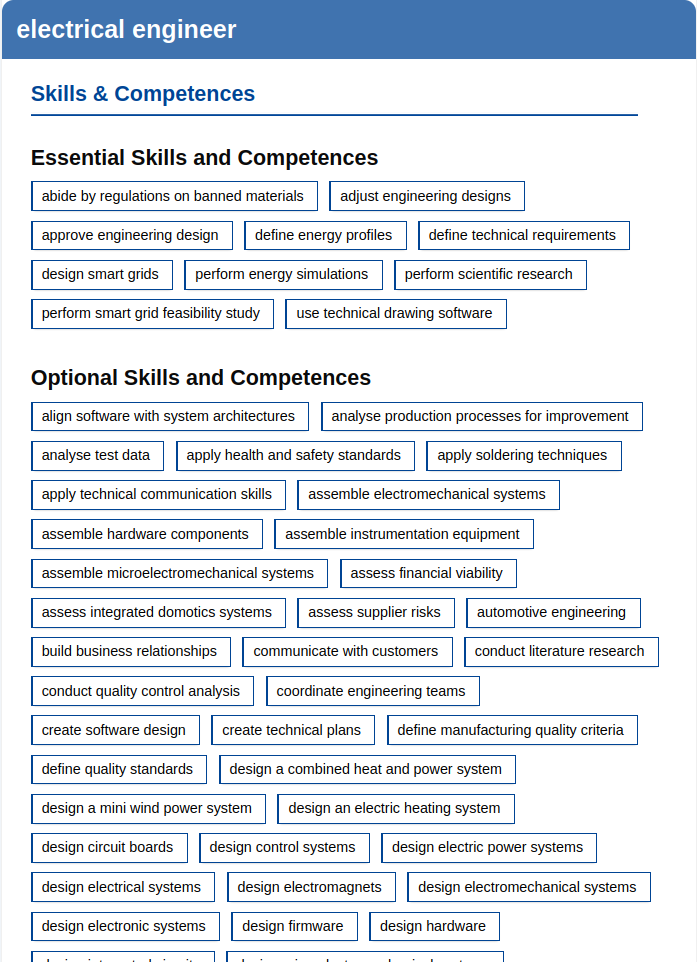
\includegraphics[width=0.95\textwidth]{img/slidesp/EE_ESCO.png}
                \label{fig:esco_eng}
            \end{figure}
        \end{column}
    \end{columns}
\end{frame}

\begin{frame}{Exposure Scores}
    \begin{columns}
      \begin{column}{0.5\textwidth}
        \begin{tcolorbox}[title=\citet{felten_method_2018}]
          Expert assessment extrapolated via a machine learning model.
        \end{tcolorbox}
        \vspace{0.5cm}
        \begin{tcolorbox}[title=\citet{eloundou_gpts_2023}]
          LLM-powred analysis using a custom prompt.
        \end{tcolorbox}
      \end{column}
      \begin{column}{0.5\textwidth}
        \begin{tcolorbox}[title=\citet{webb_impact_2022}]
          Matches patent contents to occupational skills.
        \end{tcolorbox}
        \vspace{0.5cm}
        \begin{tcolorbox}[title=\citet{demirev2024assessing}]
          Matches product announcement contents to occupational skills.
        \end{tcolorbox}
      \end{column}
    \end{columns}
\end{frame}


\begin{frame}{CEDEFOP}
    \begin{figure}
        \centering
        % Include your .png or .pdf instead of .eps if needed
        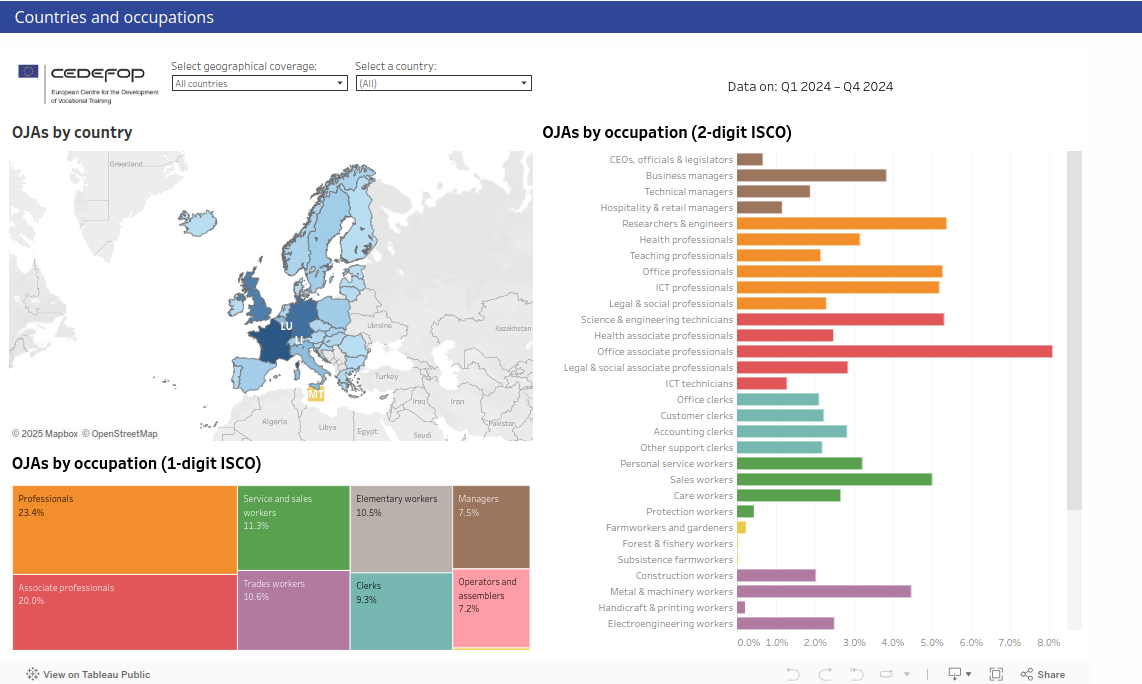
\includegraphics[width=0.95\textwidth]{img/slidesp/cedefop_dash.png}
        \label{fig:cedefop}
    \end{figure}
\end{frame}

\begin{frame}{Job Openings}
    \begin{figure}
        \centering
        % Include your .png or .pdf instead of .eps if needed
        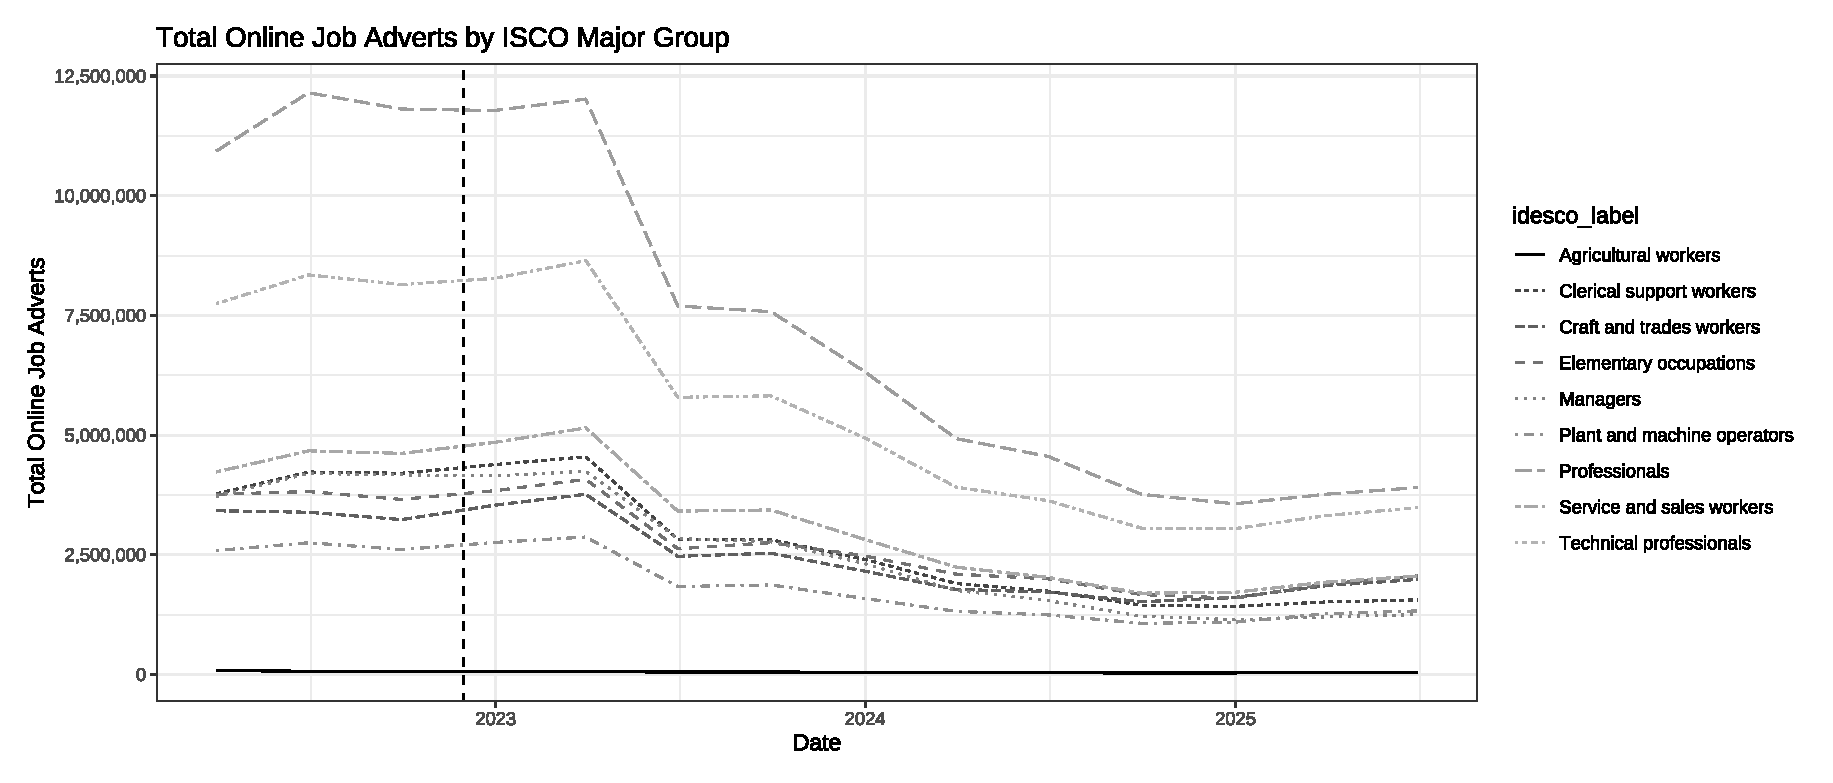
\includegraphics[width=0.95\textwidth]{img/oja_time_series.eps}
        \caption{Time series of total online job adverts across EU (Q4 2021--Q2 2024). 
        \newline \small Source: \citet{cedefop_skills_ovate} }
        \label{fig:oja_ts}
    \end{figure}
\end{frame}

\begin{frame}{Empirical Design}
    \begin{equation}
        \Delta\log{\bar{y}}_{c,i} = \delta_0 + \xi_c + \delta X_i + \varepsilon_{c,i}
    \label{eq:delta}
    \end{equation}

    \begin{itemize}
        \item Event time: release of ChatGPT (November 2022)
        \item Dependent variable: difference in average job openings pre and post the event time
        \item independent variable: any of the four exposure indices (continuous DiD)
        \item country-level fixed effects; clustered standard errors
    \end{itemize}
\end{frame}

% -------------------------------------------------------------------
\section{Results}
\begin{frame}{Main Regression Results}
    \begin{table}[H]
        \centering
        \begin{threeparttable}
        \caption{Effects of AI Exposure on Labor Demand, Productivity, and Skill Mix}
        \begin{tabular}{lcccc}
            \toprule
            & \textbf{Demirev} & \textbf{Felten et al} & \textbf{Webb} & \textbf{Eloundou et al} \\
            \midrule
            \multicolumn{5}{l}{\textbf{Labor Demand (Online Job Adverts)}} \\
            Coefficient   & $-0.186^{**}$  & $-0.138^{**}$  & $-0.174^{***}$ & $-0.193^{**}$ \\
            (SE)          & (0.056)        & (0.047)        & (0.035)       & (0.054)      \\
            Observations  & 2,817          & 2,814          & 2,805         & 2,814        \\
            Adj. $R^2$    & 0.480          & 0.479          & 0.480         & 0.482        \\
            \bottomrule
        \end{tabular}
        \begin{tablenotes}
            \footnotesize
            \item \textit{Notes:} Standard errors in parentheses. Significance levels: * $p<0.05$, ** $p<0.01$, *** $p<0.001$. All models include country fixed effects.
        \end{tablenotes}
        \label{table:models}
        \end{threeparttable}
    \end{table}
\end{frame}


\begin{frame}{Main Regression Results - Visual Illustration}
    \begin{figure}[H]
        \caption{Partial plot of AI Exposure and Online Job Adverts}
        \centering
        %\includesvg[width=0.8\textwidth,height=0.3\textheight]{visuals/research_skills_plot.svg}
        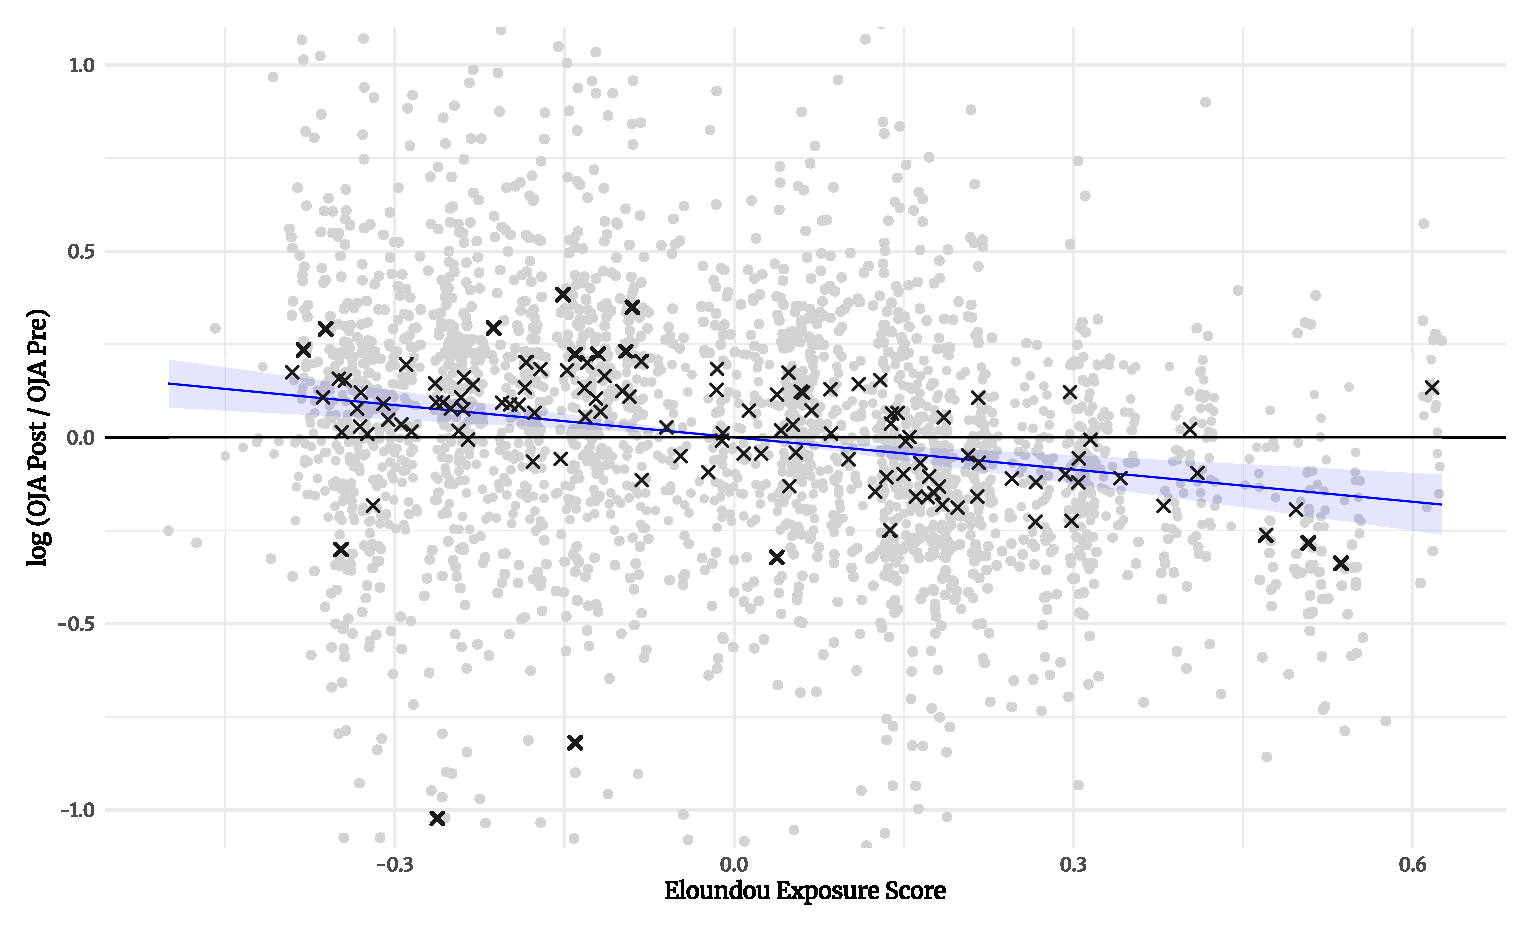
\includegraphics[width=0.6\textwidth]{img/partial_plots_eloundou.eps}
        \label{fig:partial_eloundou}
    \end{figure}
\end{frame}

\begin{frame}{Event Study}
    \begin{figure}
        \centering
        
\includegraphics[width=0.65\textwidth]{img/event_study_all.eps}
        \caption{Event-study coefficients for post-ChatGPT quarters (example for Eloundou measure).}
        \label{fig:event_study_all}
    \end{figure}
\end{frame}

\begin{frame}{Main Regression Results - Interpretation}
    \begin{itemize}
        \item Across all exposure measures, coefficients are negative and statistically significant.
        \item Moving from min to max exposure implies a roughly 13--18\% deeper decline in job postings.
        \item Within-country $R^2$ is small, implying other macro factors matter more, but the AI effect is still visible.
    \end{itemize}
\end{frame}

% -------------------------------------------------------------------
\begin{frame}{Additional Outcomes}
    \begin{columns}
        \begin{column}{0.48\textwidth}
            \begin{itemize}
                \item \textbf{Labor Productivity} Eurostat publishes quarterly data on labor productivity by sector. Combined with sectoral AI exposure metrics, we can replicate the same approach.
                \item \textbf{Skill-Level Demand} The CEDEFOP's database contains data on the number of the mentions of each skill. We can use skill-level AI exposure to examine within-occupation changes in skill demand.
            \end{itemize}    
        \end{column}
        \begin{column}{0.48\textwidth}
            \begin{figure}[H]
                %\caption{Partial plot of AI Exposure and Online Job Adverts}
                \centering
                %\includesvg[width=0.8\textwidth,height=0.3\textheight]{visuals/research_skills_plot.svg}
                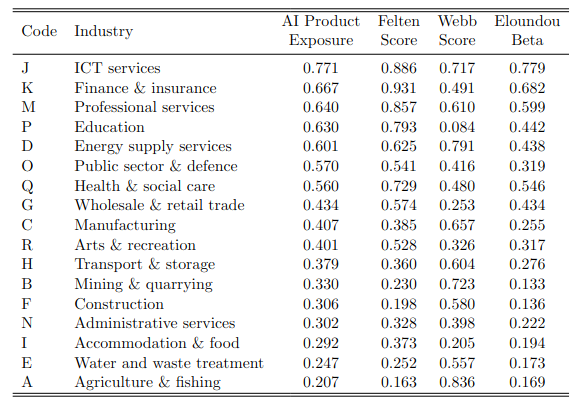
\includegraphics[width=0.99\textwidth]{img/slidesp/scores_by_industry.png}
                \label{fig:by_industry}
            \end{figure}
        \end{column}
    \end{columns}
\end{frame}

\begin{frame}{Additional Outcomes - Results}
    \begin{table}[H]
        \centering
        \begin{threeparttable}
        \caption{Effects of AI Exposure on Labor Demand, Productivity, and Skill Mix}
        \begin{tabular}{lcccc}
            \toprule
            & \textbf{Demirev} & \textbf{Felten et al} & \textbf{Webb} & \textbf{Eloundou et al} \\
            \midrule
            \multicolumn{5}{l}{\textbf{Labor Productivity}} \\
            Coefficient   & $-0.067$       & $-0.013$       & $-0.113$      & $-0.015$     \\
            (SE)          & (0.048)        & (0.025)        & (0.066)       & (0.037)      \\
            Observations  & 330            & 330            & 330           & 330          \\
            Adj. $R^2$    & 0.044          & 0.036          & 0.065         & 0.036        \\
            \midrule
            \multicolumn{5}{l}{\textbf{Skill Mix}} \\
            Coefficient   & $-0.025^{*}$   & ---            & ---           & ---          \\
            (SE)          & (0.011)        & ---            & ---           & ---          \\
            Observations  & 75,864         & ---            & ---           & ---          \\
            Adj. $R^2$    & 0.095          & ---            & ---           & ---          \\
            \bottomrule
        \end{tabular}
        \begin{tablenotes}
            \footnotesize
            \item \textit{Notes:} Standard errors in parentheses. Significance levels: * $p<0.05$, ** $p<0.01$, *** $p<0.001$. All models include country fixed effects (and occupation fixed effects in the Skill Mix model).
        \end{tablenotes}
        \label{table:models}
        \end{threeparttable}
    \end{table}
\end{frame}

\begin{frame}{Additional Outcomes - Interpretation}
    \begin{itemize}
        \item No significant effect on labor or capital productivity in 2022--2023 data.
        \item Skills with higher AI similarity see a modest but significant (2--3\%) decline in mentions, implying partial reorganization of tasks within occupations.
    \end{itemize}
\end{frame}

% -------------------------------------------------------------------
\section{Conclusion}
\begin{frame}{Conclusion}
    \textbf{Generative AI is reshaping labor markets, but the full impact is nuanced:}
    \vspace{0.5cm}
    \begin{columns}
        \begin{column}{0.58\textwidth}
            \begin{itemize}
                \item Occupations highly exposed to AI experienced significant decreases (13--18\%) in labor demand.
                \item Specific skills resembling AI capabilities faced reduced demand within occupations.
                \item Overall, AI is far from the main driver of recent labor market dynamics.
                \item No clear evidence (yet) of significant productivity gains at the industry level, hinting at "so-so automation".
            \end{itemize}
        \end{column}
        \begin{column}{0.38\textwidth}
            \begin{figure}
                \centering
                % Include your .png or .pdf instead of .eps if needed
                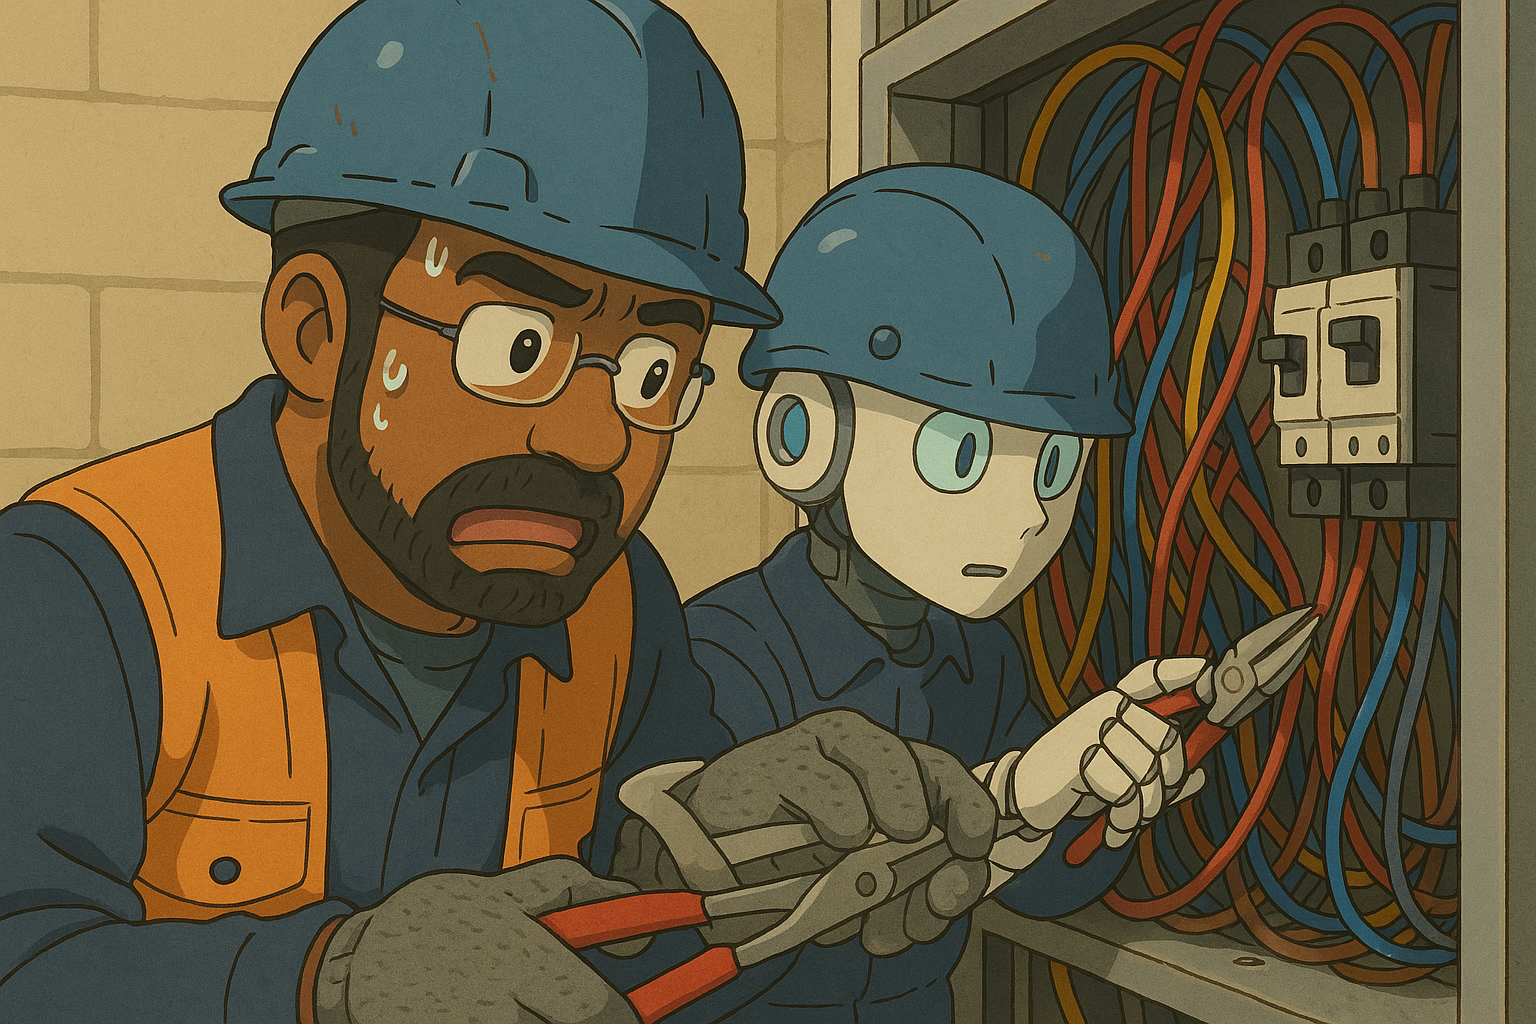
\includegraphics[width=0.99\textwidth]{img/slidesp/ee_ai_anime.png}
                \label{fig:ai_ee}
            \end{figure}    
        \end{column}
    \end{columns}
\end{frame}

\begin{frame}{Limitations and Future Work}
    \begin{itemize}
        \item \textbf{Data coverage and “ghost postings”} in online adverts can bias results.
        \item Potential \textbf{pre-trends} and endogeneity issues in difference-in-differences.
        \item Productivity data is not granular enough
        \vspace{0.5cm}
        \item \taxtbf{Future research and policy implications:} 
        \begin{itemize}
            \item Monitoring shifts in skill demands is essential for targeted upskilling initiatives.
            \item Further research needed on long-term productivity and employment effects.
            \item Discerning between complementary vs. displacement tasks
        \end{itemize}
    \end{itemize}
\end{frame}

% -------------------------------------------------------------------
\section{References}
\begin{frame}[allowframebreaks]{References}
\tiny
\bibliographystyle{plainnat}
\bibliography{references}
\end{frame}

\end{document}
